% A (little more than a) minimal working example
\documentclass[12pt, a4paper]{article}

% Increase tex widht and heigh by 4cm
\addtolength{\textwidth}{4cm}
\addtolength{\oddsidemargin}{-2cm}
\addtolength{\textheight}{4cm}
\addtolength{\topmargin}{-2cm}

% To start out let's include the following packages
\usepackage[utf8]{inputenc} % encoding
\usepackage{hyperref} % for clickable references
\usepackage{xcolor} % custom colors
\usepackage{graphicx} % for including graphics
\usepackage{pgfplots} % for plots and more
\usepackage{tikz} % for drawing and more
\usepackage{booktabs} % for nice tables
\usepackage{amsmath} % math stuff
\usepackage{amsfonts}
\usepackage{amssymb}

\begin{document}

\title{%
  {\bfseries Main Title}\\[1ex] % your title goes here
  {\large\bfseries Subtitle} % if you want to use a subtitle...
}
\author{ Max Mustermann} % your name

\date{\vspace{-5ex}} % dirty hack to remove date from titlepage

{\sf \maketitle} % use serif free font for title page

\begin{center}
  
\includegraphics[width=8cm]{logo_sdv.pdf}\\
  {\large\sf Sommerakademie in Leysin, August 2016}
\end{center}

\vspace{1cm}

\begin{abstract}
  A short description of the article.
\end{abstract}

% The table of contents
\newpage
\tableofcontents

\newpage
\section{Introduction}\label{sec:introduction}

This is just some sample text for illustration purposes. We figured that you
probably belong to one of the following groups
\begin{enumerate}
  \item You are a \LaTeX{} expert, know how to use it, all necessary commands
  and have used it extensively to typeset documents. In this case you don't need
  our advice and we simply ask you to use this template for the purpose of
  having a uniform layout.
  \item You have limited \LaTeX{} experience. You have already played around a
  little bit or compiled a few documents at some point.
  \item You have heard about it, but never used it yourself.
  \item What is \LaTeX{}?
\end{enumerate}
If you belong to one of the latter 3 groups, we strongly encourage you to get to
know (and love) \LaTeX{}. We do not expect you to use \LaTeX{} for this summer
academy, but mastering \LaTeX{} is an incredibly valuable -- if not necessary --
skill. The sooner you get on it, the better.

We cannot provide an introduction to typesetting documents with \LaTeX{} here,
there is plenty of good material on the internet. In particular, we will not go
into the details of how to compile a \LaTeX{} docmuent. However, we decided to
fill this template with a diverse mixture of commands and \LaTeX{} showcases.
This might serve as a reminder of the syntax and commands for the people in the
second group, point members of the first group to interesting advanced packages
and could also be a complementary starting point for people who have never used
it. If you have any questions about this template, the compilation process or
\LaTeX{} in general feel free to shoot us an email anytime. That said, let's get
started!

First, we include a simple equation
\begin{equation} \label{einstein}
  R_{\mu \nu} - \frac{1}{2} R g_{\mu \nu} + \Lambda g_{\mu \nu} = \frac{8 \pi
  G}{c^4} T_{\mu \nu} \: .
\end{equation}
We can later refer to that equation like this~\eqref{einstein}. The \texttt{\~}
in the source is just an unbreakable space to prohibit a line break at that
position. We can also refer to different sections, for example
section~\ref{sec:empty}, or section~\ref{sec:new}.

A blank line creates a new paragraph.

If we do not want the equation to have a number, we can use the ``starred''
version of the \texttt{equation} environment, e.g.
\begin{equation*}
  \hat{H} | \psi(t) \rangle =
  i \hbar \frac{\partial}{\partial t} | \psi (t) \rangle \: .
\end{equation*}

As an alternative to the starred version, we can also use the shorter version
\[
  \int_M K dA + \int_{\partial M} k_g ds = 2 \pi \chi (M) \:.
\]

Of course, inline math expressions are not problem either:~$\pi =
\sum_{k=0}^{\infty} (3^k - 1) \zeta (k + 1) / 4^k$.
Let us do something more fancy
\begin{align}
  \nabla \cdot E &= \frac{\rho}{\epsilon_0} \label{max1} \\
  \nabla \cdot B &= 0 \label{max2} \\
  \nabla \times E &= - \frac{\partial B}{\partial t} \label{max3} \\
  \nabla \times B &= \mu_0
  \left(J + \epsilon_0 \frac{\partial E}{\partial t} \right) \: . \label{max4}
\end{align}
Here we have four equations~\eqref{max1}, \eqref{max2}, \eqref{max3},
and~\eqref{max4}.

The indicator function of the rational numbers~$\chi_{\mathbb{Q}}: \mathbb{R} \to
\mathbb{R}$ is defined by
\begin{equation}\label{indicator}
  \chi_{\mathbb{Q}}(x) :=
  \begin{cases}
    1 &\text{if } x \in \mathbb{Q} \\
    0 &\text{if } x \in \mathbb{R} \setminus \mathbb{Q} \\
  \end{cases}
\end{equation}
is Lebesgue integrable with integral~$\int_{\mathbb{R}} \chi_{\mathbb{Q}}
d\lambda = 0$, but is not Riemann integrable.

\section{A new section}\label{sec:new}

If we want to cite other papers, we write a separate file,
e.g.~\texttt{paper.bib}. It contains the metadata of the work we want to cite in
a special format called
\href{https://en.wikipedia.org/wiki/BibTeX}{\emph{bibtex}}. When looking up
references online, you will often be able to copy paste citations in the bibtex
format. To refer to such a bibtex entry in our \texttt{paper.tex} document, we
type
\texttt{\textbackslash{}cite\{<name of entry in paper.bib>\}}, which results
in something like this:~\cite{idatacool}. The bibliography is included at the
very end of the document.

We love pictures. Let us include that logo of the Studienstiftung again, which
we have already seen on the title page. We included it as
figure~\ref{fig:logosdv}.
\begin{figure}
  \begin{center}
    
\includegraphics[width=8cm]{logo_sdv.pdf}
  \end{center}
  \caption{The official new logo of the Studienstiftung. Looking good!
  \label{fig:logosdv}}
\end{figure}
\LaTeX{} usually does a good job positioning the figures on its own if there is
enough text around. Note that they will not necessarily show up exactly where
you put them in the document. In particular in this short template, they will
all be crammed together in weird places. For more manual control check out
\href{https://en.wikibooks.org/wiki/LaTeX/Floats,_Figures_and_Captions}{this
link}.

Because pictures are so cool\footnote{By the way, footnotes are really easy in
\LaTeX{} too!}, let's unleash the awesomeness of
\href{http://www.ctan.org/pkg/pgfplots}{pgfplots} and
\href{http://www.ctan.org/pkg/pgf}{TikZ}. This is a little bit more advanced and
is definitely a challenge for unexperienced \LaTeX{} users. However, the
learning curve is steep and it is truly worth the effort. We both love TikZ and
pgfplots.  For some cool examples click
\href{http://www.texample.net/tikz/examples/all/}{here} or
\href{http://pgfplots.sourceforge.net/gallery.html}{here}.

Figure~\ref{fig:tikz} shows a little sample picture produced with
TikZ\footnote{Fun fact: TikZ is a recursive acronym for \textbf{T}ikZ
\textbf{i}st \textbf{k}ein \textbf{Z}eichenprogramm.} that we have stolen from
the website mentioned above. Figure~\ref{fig:plot} shows plots created with
pgfplots (also stolen of course).

\begin{figure}
  \begin{center}
  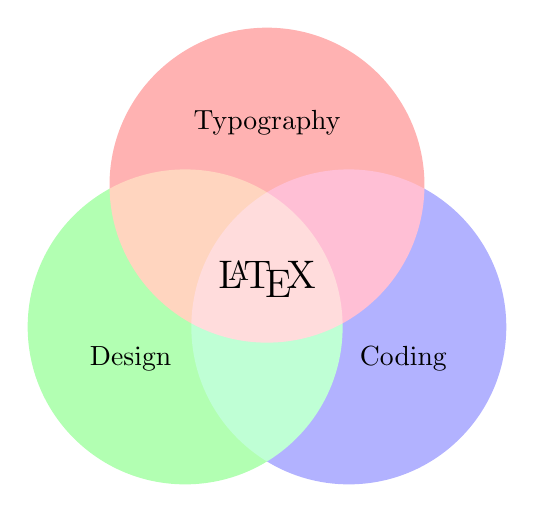
\begin{tikzpicture}
    \begin{scope}[blend group = soft light]
      \fill[red!30!white] ( 90:1.2) circle (2);
      \fill[green!30!white] (210:1.2) circle (2);
      \fill[blue!30!white] (330:1.2) circle (2);
    \end{scope}
    \node at (90:2) {Typography};
    \node at (210:2) {Design};
    \node at (330:2) {Coding};
    \node [font=\Large] {\LaTeX{}};
  \end{tikzpicture}%
  \end{center}
  \caption{Sweet huh?\label{fig:tikz}}
\end{figure}

\begin{figure}
  \begin{center}
  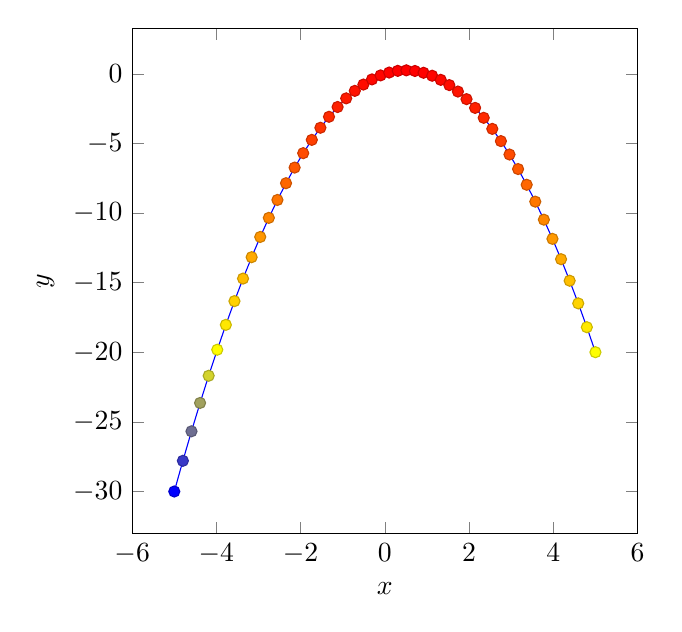
\begin{tikzpicture}
    \begin{axis}[
        width={8cm},
        height={8cm},
        xlabel={$x$},
        ylabel={$y$},
      ]
      \addplot+[scatter, samples=50,scatter src=y] {x-x^2};
    \end{axis}
  \end{tikzpicture}%
  \hfill
  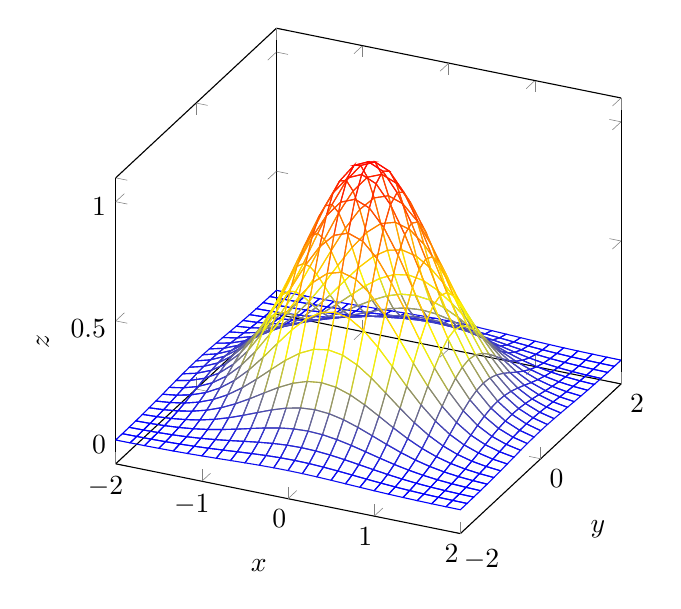
\begin{tikzpicture}
    \begin{axis}[
        width={8cm},
        height={8cm},
        xlabel={$x$},
        ylabel={$y$},
        zlabel={$z$},
      ]
      \addplot3[mesh, domain=-2:2] {exp(-x^2-y^2)};
    \end{axis}
  \end{tikzpicture}%
  \end{center}
  \caption{Best option for publication quality plots.\label{fig:plot}}
\end{figure}

\section{An empty section} \label{sec:empty}

Nothing in this section \dots

\subsection{Just ignore this} \label{subsec:ignore}

\dots except for this one subsection.

\subsection{Ignore this too} \label{subsec:ignoretoo}

We just need to fill the table of contents.

\section{The end} \label{sec:end}

Almost as nice as pictures and plots are tables. It is increadibly easy to screw
up tables in \LaTeX{}\footnote{Read the introduction of the \texttt{booktabs}
manual or check out
\href{https://www.inf.ethz.ch/personal/markusp/teaching/guides/guide-tables.pdf}
{these slides}.} and the very basic inbuilt commands make it hard for the user
to create truly beautiful tables. The de-facto standard solution to this is the
\href{https://www.ctan.org/pkg/booktabs}{\texttt{booktabs}} package, which we
have already included in our little sample document. Table~\ref{tab:sample} is
an example of what tables should look like.

\begin{table}
\begin{center}
    \begin{tabular}{@{} l *4c @{}}
    \toprule
    \multicolumn{1}{c}{Models}    & A  & B  & C  & D  \\
    \midrule
    Model $X$ & X1 & X2 & X3 & X4 \\
    Model $Y$ & Y1 & Y2 & Y3 & Y4 \\
    \bottomrule
    \end{tabular}
  \end{center}
  \caption{Some groundbreaking new results displayed as a table.
  \label{tab:sample}}
\end{table}

% References
\bibliographystyle{plain}  % you can try 'alpha' or 'abbrv' instead of 'plain'
\bibliography{paper} % references are found in the file `paper.bib`

\end{document}
